\documentclass[10pt,a4paper]{article}
\usepackage[utf8]{inputenc}
\usepackage{amsmath}
\usepackage{amsfonts}
\usepackage{amssymb}
\usepackage{todonotes}
\usepackage{graphicx}

\graphicspath{{img/}}

\author{150016853}
\title{CS5011 - P4}
\begin{document}
\maketitle

\section{Overview}

A specification has been provided in which multiple bayesian networks have been constructed and analysed. 

\begin{itemize}
\item Built networks to specification
\item Added 2 additional events to network
\item Evaluated influence on adding events using 3 different queries
\end{itemize}
\todo{list implementated parts}
\todo{literature review}


\section{Part 1 Design Procedure}

The primary procedure for design focussed on segmentation and semantics: At each point of construction, required for the given network,  establishing the causal chain of probabilities that most accurately correlate to the English representation of the problem. More importantly creating causal chains which don't correspond directly to the English interpretation intuitively. 

Another focus in the design decisions was the distinction between implicit and explicit declaration of variables through events. For example if we were to put in an event which was the receipt of an email and that email can be one of a business or personal email, the inclusion of an event describing if that email is a business email can potentially remove the requirement to include an event expressing that a personal email has arrived, given that it is implicit that since an email has arrived and it is not a business email that is must therefore be a personal email. This, however may limit how we express our queries, where a more expressive query is often easier to understand. That being said it does also increase the set of events we require to fully describe our network. For this specification it has been decided that an explicit declaration of our variables through inclusion of more nodes in our graphs was more appropriate, especially given the small scale of the networks to be implemented.

Once we have the set of relation and events it is typically fairly easy to intuit the form the CPT should take for each node.

\subsection{Email Risk Assessment}
To begin implementing the specified networks we consider the causal chain that results in a set of digestible, useful events defined across our network. Let us consider the email section of our specified network. 

Let us break our specified problem into distinct events through which we can create a causal chain that our network can represent.

\begin{itemize}
\item We can received an email that is one of a business or personal email
\item We can categorise this email as high or low risk - high if personal, low if business
\item The system can fail to correctly categorise this email with a 3\% probability
\end{itemize}

If we segment these into more digestible chunks we can get

\begin{itemize}
\item We can receive an email
\item We can categorise this email as business
\item We can categorise this email as personal if the email is not a business email
\item We can categorise personal emails as high risk
\item The system can fail to correctly categorise an email
\item The system can flip the correct categorisation of an email due to misinformation errors
\end{itemize}

These allow us to construct a set of relations and events(Fig. \ref{fig:email_network}) which tie well into our English understanding of the problem domain.

\begin{figure}
\centering
  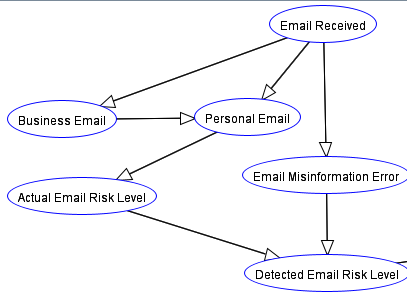
\includegraphics{email_network.png}
  \caption{Email Bayesian Network.}
  \label{fig:email_network}
\end{figure}


By expanding this procedure to the full specification we requested we can establish a set of events and relations for each distinct segment of the problem space.

\subsubsection{CPT}

A initial probability of receiving an email has been set and 0.99. This is given that across a company we would typically expect a largely continuous stream of emails being received. Given this we defined a 0.9 probability that an email is business and as such implicitly a 0.1 probability that an email received is personal. Again we should expect a company to receive overwhelmingly business emails.

As such the risk level can be determined using binary 100\% or 0\% chances to be raised, given we know whether a personal email has been received. 

The email misinformation error can be raised only if an email is received and has a probability of 3\% of being raised, as specified.

The detected Email Risk Level acts as a Not gate for the output on the Actual Email Risk Level, given that the Email Misinformation Error node outputs true.

\subsection{Maintenance Risk Assessment}

\begin{itemize}
\item Maintenance may be planned
\item If maintenance is planned the firewall may go down
\item Maintenance information may be out of date
\item If maintenance information is out of date and maintenance information is planned the system is considered vulnerable
\item If the firewall is down or vulnerable due to maintenance information being out of date the system is considered high risk.
\end{itemize}

The specified "additional 2\%" chance of vulnerability due to maintenance information being out of date has been interpreted as referring to a distinct vulnerability from the possibility for the firewall being down and instead is a second possibility for vulnerability when maintenance is planned. As such the "Maintenance Information Out of Date" node has a 2\% chance of being true.

\begin{figure}
\centering
  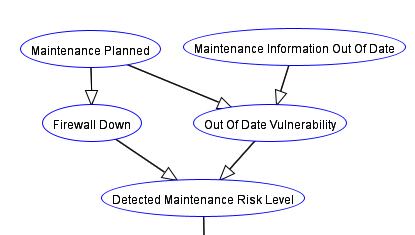
\includegraphics{maintenance_network.png}
  \caption{Maintenance Bayesian Network.}
  \label{fig:maintenance_network}
\end{figure}

\subsubsection{CPT}

Maintenance plan has a 20\% chance of being true, from which Firewall Down has a 0\% chance of being true if no maintenance is planned and 5\% chance otherwise.

Maintenance info being down has a 2\% chance of being true, given maintenance is planned and this info is out of date there is a 100\% chance of vulnerability.

Given either Firewall Down or Out Of Date Vulnerability is true Detected Maintenance Risk Level is guaranteed true, otherwise false.

\subsection{Days Risk Assessment}

\begin{itemize}
\item It can be a holiday or political day.
\item If it is a holiday or political day it is considered a high risk day.
\end{itemize}

\begin{figure}
\centering
  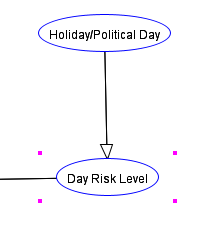
\includegraphics{day_network.png}
  \caption{Day Risk Bayesian Network.}
  \label{fig:day_network}
\end{figure}

\subsubsection{CPT}

Holiday/Political day has a 100/360 chance of being true. Given Holiday/Political Day is true, Day Risk Level is high, otherwise low.

\subsection{Logging Response}

\begin{itemize}
\item A high risk alert can be triggered
\item Following a high risk alert an investigation occurs
\item An investigation can rule that the alert was anomalous
\item If an investigation does not rule that it was anomalous it will rule that it was normal instead
\item If an investigation occurs their conclusion may be incorrectly logged
\item If an investigation rules that the alert was anomalous it will log anomalous, unless a logging error occurs. If an investigation rules that the alert was not anomalous the system will not log anomalous, unless a logging error occurs.
\item If an investigation rules that the alert was normal it will log anomalous, unless a logging error occurs. If an investigation rules that the alert was not normal the system will not log anomalous, unless a logging error occurs.
\end{itemize}

\begin{figure}
\centering
  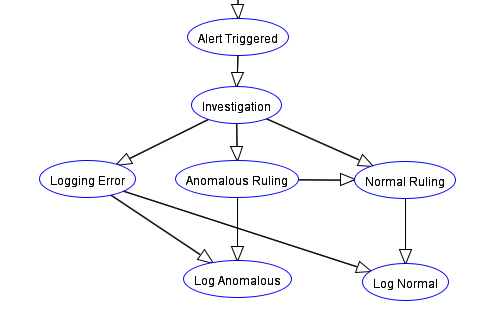
\includegraphics{logging_network.png}
  \caption{Loggin Response Bayesian Network.}
  \label{fig:logging_network}
\end{figure}

\subsubsection{CPT}

Given a Alert Triggered, investigation has 100\% chance of being true, otherwise false. If Investigation is true, Logging Error has a 30\% chance of being true, otherwise a 0\% chance. Anomalous ruling has a 10\% chance of being true, otherwise 0\%. Given anomalous ruling is true, normal ruling is never true. Given there is an investigation and anomalous is not true normal ruling must be true.

For Log Anomalous and Log Normal given their respective ruling and no error or if not their respective ruling and an error they are true. Otherwise they are false.

\subsection{Alerting}

\begin{itemize}
\item If there is deemed a high email risk, a high maintenance risk or high day risk the overall system will be considered high risk.
\item If the system is high risk an alert will be triggered
\end{itemize}

\begin{figure}
\centering
  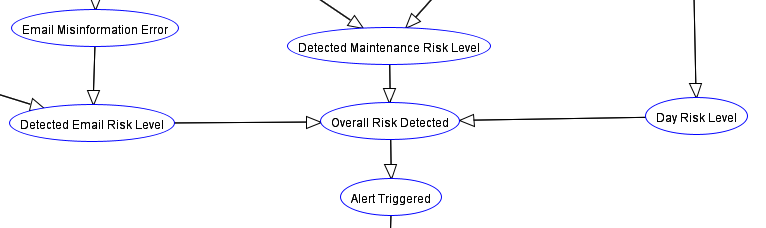
\includegraphics[width = \linewidth]{alarm_network.png}
  \caption{Alerting Bayesian Network.}
  \label{fig:alerting_network}
\end{figure}

\subsubsection{CPT}

The CPT essentially is an inclusive OR. If any of the parent nodes are true the Overall Risk Detected is high and as such an Alert is triggered.

\todo{network 2}

\subsection{Extending Network}

Our network has been expanded to include two more events. An event is included where a business email received may be from a forbidden domain with a 5\% probability. If this is the case it is considered high risk of attack (Fig. \ref{fig:flagged_forbidden}).

\begin{figure}
\centering
  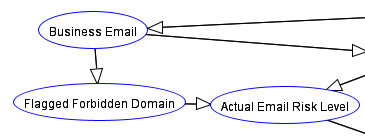
\includegraphics{flagged_forbidden.png}
  \caption{Flagging Additional Event.}
  \label{fig:flagged_forbidden}
\end{figure}

An event is also included wherein with low frequency (1\% probability) the bureaucracy can fail, leading to an investigation never occurring after an alert has been raised (Fig. \ref{fig:bureaucratic_failure}).



\begin{figure}
\centering
  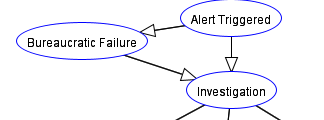
\includegraphics{bureaucratic_failure.png}
  \caption{Bureaucratic Failure Additional Event.}
  \label{fig:bureaucratic_failure}
\end{figure}

\section{Part 1 Evaluation}

\subsubsection{Predictive}

Given that an alarm was triggered what is the probability that an anomalous log is made.

Across the first network it was found that there was a 34\% chance of an anomalous log, given that an alert occurred.

In our second network it was found that there was a 33.6\% chance that given an alert occurred that an anomalous log occurred. This intuitively makes sense, given that we would expect a decrease in the likelihood of an investigation happening if there is bureaucratic failure and as such lower chance that anything would be logged.

\subsubsection{Diagnostic}

Given that there is a high risk of email attack detected, what are the chances that a business email was received.

Across the first network it was found that there was a 21\% chance of having received a business email, given that there was detected a high risk of attack.

Across the first network it was found that there was a 41\% chance of having received a business email, given that there was detected a high risk of attack. This intuitively makes sense, given that we have added another means by which business emails can be flagged as high risk by including flagging of banned domains.

\subsubsection{Profiling}

Let us consider the alert event for profiling. First allow us to consider when it is set true. We can guarantee that if it is true at least one of the detected email risk level, detected maintenance risk level or day risk level is high. If we run several queries across these events to establish the probability that given an alert occurs what is the chance we were in a high risk state across one of the risk levels we can establish the most likely high risk event leading to an alert being triggered, as well as the least likely. In running these queries we can determine that across network 1 with a 74.0\% chance of having occurred a high risk day was the most likely to be the case when an alert was triggered. Second to this was an email attack risk with a 32.7\% chance of being high risk and then maintenance attacks with a 3.7\% chance of being high risk when an alert is triggered.

We can then observe how this changes across our two additional networks. For our second network we see that as we include our additional email event allowing business emails to be flagged as high risk we see the probability that the email attack was true given the alert happen increase to a 40.7\% chance across network 2 whilst the other 2 decrease, with maintenance risk dropping to a 3.4\% chance and day risk dropping to 68.6\% chance.

Conversely if we look at the probability of any being high risk given no alert was triggered we can observe across all networks a slight chance that the alert has not occurred despite the fact a high risk status has been defined. With email attacks being true despite no alert at a 3.5\% across network 1 chance and 4.9\% chance across network 2, high risk days being true despite no alert at 8.9\% for network 1 and increasing to 8.2\% across network 2 and finally at 0.4\% for network 1 and remaining ~the same at 0.4\% for network 2 for maintenance risk.
                                                             
In then looking at the consequences of an alert being triggered, our probably most useful outcome to observe may be the likelihood that an anomalous or normal logging will occur. So we shall run diagnostic queries along these lines to establish the consequences of an alert being raised. We can see that for our initial network there is a 34.0\% chance that given an alert was triggered that an anomalous ruling will be logged and a 66.0\% chance that a normal ruling will be logged. Conversely if we consider the condition on which an alert triggered is false we see that there is a 0\% probability both for it to log anomalous results and log normal results, this behaviour matches the intended specification.

\section{Part 2}

\subsection{Merging Algorithm}

A full merging algorithm has been implemented including unit tests to demonstrate functionality. 
\subsubsection{Design}

The system uses Encog networks as inputs, deconstructs them to a set of dependencies and probability tables then eliminates and combines dependencies/tables via usage of variation on Feng et al (2014) algorithm as highlighted in lecture slides\cite{feng}.

A note of design consideration is in the requirement to retranslate our newly merged network to Encog we must preserve the order that the original networks understood the order of the arguments in the CPT. This allows us to correctly align our new CPT  probabilities with the correct set of inputs when combining probabilities.
\todo{talk about corner case}
\subsubsection{Testing}

A test suite has been provided which covers examples of merging simple networks.

\subsubsection{Example 1}

Consider an example execution from one of our tests.

We can see the form of our two initial networks as a pair of single dependency networks with a common node in C (Fig. \ref{fig:ex1_init_a}/\ref{fig:ex1_init_b}).
\begin{figure}
\centering
  \includegraphics{ex1_init_a.png}
  \caption{Example Network Combination A Network.}
  \label{fig:ex1_init_a}
\end{figure}

\begin{figure}
\centering
  \includegraphics{ex1_init_b.png}
  \caption{Example Network Combination B Network.}
  \label{fig:ex1_init_b}
\end{figure}

Our merger identifies the intersection on C as well as that C is an external node given neither B nor A is in the intersection (Fig.\ref{fig:ex1_id_elem}).

\begin{figure}
\centering
  \includegraphics{ex1_id_elem.png}
  \caption{Example Network Intersection Identification.}
  \label{fig:ex1_id_elem}
\end{figure}

We then observe the beginning of the addition to the new merged network (Fig. \ref{fig:ex1_comb_elem}). We observe that C is handled using ZE procedure with the probability product being produced for all combination of inputs across the node (Fig.\ref{fig:ex1_comb_prob}). The resulting probabilities are normalised via the sum of their probabilities in the table line(Fig.\ref{fig:ex1_norm_prob}).

\begin{figure}
\centering
  \includegraphics{ex1_comb_elem.png}
  \caption{Example Network Combination.}
  \label{fig:ex1_comb_elem}
\end{figure}

\begin{figure}
\centering
  \includegraphics[width=\linewidth]{ex1_comb_prob.png}
  \caption{Example Probability Combination.}
  \label{fig:ex1_comb_prob}
\end{figure}

\begin{figure}
\centering
  \includegraphics[width=\linewidth]{ex1_norm_prob.png}
  \caption{Example Probability Normalisation.}
  \label{fig:ex1_norm_prob}
\end{figure}


There is no requirement to prune duplicate elements(Fig.\ref{fig:ex1_prune_dep}). This resulting network is of the form we would expect across this merge with c having two new parents of which their CPT is the combination of the originals\ref{fig:ex1_comb_net}.

\begin{figure}
\centering
  \includegraphics{ex1_prune_dep.png}
  \caption{Example Pruning Avoidance.}
  \label{fig:ex1_prune_dep}
\end{figure}

\begin{figure}
\centering
  \includegraphics{ex1_comb_net.png}
  \caption{Example Combined Networks.}
  \label{fig:ex1_comb_net}
\end{figure}


\subsubsection{Example 2}

Let us consider our initial networks. An intersection of 2 nodes, on c and b, where c is dependent only on our root, as such being an inner node, and b is dependent on a or b, network dependent and c in both networks, making it an external node(Fig. \ref{fig:ex2_init_a}/\ref{fig:ex2_init_b}).
\begin{figure}
\centering
  \includegraphics{ex2_init_a.png}
  \caption{Example 1 Network Combination A Network.}
  \label{fig:ex2_init_a}
\end{figure}

\begin{figure}
\centering
  \includegraphics{ex2_init_b.png}
  \caption{Example 2 Network Combination B Network.}
  \label{fig:ex2_init_b}
\end{figure}

The program identifies this(Fig. \ref{fig:ex2_id_elem}) and proceeds as before. However in this instance we have the case of pruning being required. Given that we would typically construct a probability table composed of all arguments combined across all possible values as our new probability table values, there are examples where this is impossible. In this case there would exist lines in the CPT where C could be both true and false. These lines are removed and the additional column in the arguments are removed as well.

\begin{figure}
\centering
  \includegraphics{ex2_id_elem.png}
  \caption{Example 2 Network Intersection Identification.}
  \label{fig:ex2_id_elem}
\end{figure}

\begin{figure}
\centering
  \includegraphics{ex2_prune_dep.png}
  \caption{Example 2 Network Pruning Dependencies.}
  \label{fig:ex2_prune_dep}
\end{figure}

\subsubsection{Evaluation}

The code provided covers all cases tested. There are some pieces of inefficient code that would be better to optimise and  it would be preferable to make it more object-oriented.

\section{Literature Review}

Bayesian networks have been applied in a wide variety of contexts, being widely used in machine learning research.

It is popular partially due to it's flexibility and it's demonstrably high performance against neural networks for multiple classification tasks\cite{book}.

For example it's usage extends into providing quick queries but with approximate answers, utilising relations and independences between variables of the database to perform imperfect count queries quickly\cite{book}.

In Medicine Gene Regulatory Networks are molecular regulators which play a role in the production of body structures and as such is useful information to study to understand the body. It was found that Bayesian Networks could better model the structure of these networks than previous methods\cite{gene}.

Alternate uses include biomonitoring to establish the quality of river water, for example by modelling the animal and plant life within a river to establish the health of the river. It was found that Bayesian significantly outperformed the former methods of doing so\cite{biomonitoring}.

\section{Part 3}

An expert system for querying the bayesian network provided in part 2 has been created. One may query it using formal definitions of queries. 

\begin{thebibliography}{9}
\bibitem{feng} 
Feng G., Zhang J., Liao S., 
\textit{A novel method for combining Bayesian networks, theoretical
analysis, and its applications.} Pattern Recognition, 2014
 
\bibitem{book}
Mittal, Ankush, ed. Bayesian Network Technologies: \textit{Applications and Graphical Models: Applications and Graphical Models}. IGI Global, 2007.

\bibitem{genes}
Yue Fan, Xiao Wang, and Qinke Peng, \textit{“Inference of Gene Regulatory Networks Using Bayesian Nonparametric Regression and Topology Information,”} Computational and Mathematical Methods in Medicine, vol. 2017, Article ID 8307530, 8 pages, 2017. https://doi.org/10.1155/2017/8307530.

\bibitem{biomonitoring}
Walley, W. J., and Sašo Džeroski. \textit{"Biological monitoring: a comparison between Bayesian, neural and machine learning methods of water quality classification."} Environmental Software Systems. Springer, Boston, MA, 1996. 229-240.
\end{thebibliography}

\end{document}